\section{绪论}\label{sec:introduction}

\subsection{研究背景}

遥感图像中的船舶检测，是海上监管、港口调度、海事执法与应急救援等应用中的基础环节。和自然场景目标检测相比，遥感图像的视野更大、背景更杂、目标更稀疏，尺度变化也更明显。依赖人工判读时，效率、一致性和可追溯性都不理想。随着深度学习目标检测技术的发展，将其引入遥感船舶检测任务，并继续把结果组织成可复验、可演示、可回放的系统链路，已经有了比较明确的研究和应用价值。

近年来，目标检测技术从 two-stage 走到 one-stage、anchor-free，再到 transformer 检测器，模型在精度、速度和表达能力上持续演进\cite{ren2015_fasterrcnn,lin2017_fpn,lin2017_focalloss,tian2019_fcos,redmon2016_yolo,carion2020_detr,zhu2021_deformabledetr}。与此同时，遥感小目标检测也一直在关注尺度变化、背景干扰和样本稀疏对模型稳定性的影响\cite{wang2023_sod_review,zhao2024_shipsurvey}。不过，在中分辨率遥感图像中，微小船舶占据的像素本就有限，还容易和海浪、云层、岸线或近岸建筑纹理混在一起，通用检测器直接迁移时往往会出现漏检和误检。

公开数据集和开源工具链逐步完善后，问题也从“模型能否训练出来”转向“结果能否统一评测、稳定复现并进入可运行流程”。只给出单一模型指标已经不够，仍需要在同一协议下比较不同检测范式，并把算法能力接入系统。本文的工作就是在这个背景下展开的。

\subsection{研究问题与挑战}

本课题讨论的是“遥感场景下的微小船舶检测系统设计与实现”。实际要解决的问题并不是单纯把某个模型的 AP50 做高，而是在弱纹理目标、复杂背景和可运行系统之间找到一个能解释得通的取舍。结合 LEVIR-Ship 数据集的图像特征以及 DRENet 等已有工作\cite{chen2022_tinyship_drenet}，本文把问题拆成以下几个较具体的难点。

首先是尺度问题。微小船舶在整幅图中只占很少像素，特征图经过多次下采样后，可用于定位的细节更少。其次，海浪、云层、岸线和港区设施会形成大量近似船体的小纹理，模型一旦把这些纹理当作候选目标，Precision 就会明显受影响。再次，LEVIR-Ship 中不同图像块的目标密度、朝向和局部对比度差异较大，训练时正负样本比例并不稳定。还有一个容易被忽略的问题：数据划分、输入尺寸、阈值和评测脚本只要不一致，跨模型比较就会变得很难解释。

基于这些情况，本文不把工作写成一次单模型调参，而是同时保留实验协议、多模型比较和系统联调三条线。这样做步骤更杂，但结论来源更容易追溯，答辩时也能用系统结果核对离线实验结果。

\subsection{研究目标与主要内容}

本文的目标可以概括为：围绕 LEVIR-Ship 数据集，整理一套可复查的数据和评测口径，完成 DRENet、FCOS 与 YOLO26 的对比实验，并把可用的推理能力接入到一个本地 Web 系统中。论文写作、实验表格和系统页面尽量使用同一批结果，避免出现“论文一套、系统一套”的情况。

具体工作包括：

\begin{enumerate}
      \item \textbf{整理数据与评测口径}：固定数据划分、指标计算方式和结果记录字段，减少模型比较中的人为差异；
      \item \textbf{完成三类模型实验}：围绕 DRENet、FCOS 与 YOLO26，记录训练、测试和正式结果，比较不同检测路线的表现；
      \item \textbf{补充误差与消融观察}：结合阈值、输入尺寸和可视化样例，分析误检、漏检以及尺度敏感性差异；
      \item \textbf{搭建检测系统原型}：采用 React、FastAPI 与 SQLite 接入本地推理能力，实现任务提交、异步执行、结果保存和历史回看。
\end{enumerate}

\subsection{本文主要工作与贡献}

结合目前完成的实验和系统，本文的工作重点主要体现在以下三方面。

第一，围绕遥感微小船舶检测任务，本文整理了数据组织和评测记录方式。数据划分、输入口径、评价指标和结果字段被放到同一套约束下，后续表格中的模型差异才有相对稳定的比较基础。

第二，本文完成了 DRENet、FCOS 与 YOLO26 的对比实验，并把阈值消融、输入尺寸敏感性和定性样例放在一起阅读。这样处理后，AP50 接近但 Precision、Recall 差别很大的情况就不再只是表格中的数字，而可以对应到具体错误类型和部署取舍。

第三，本文将离线推理能力封装到前后端分离的轻量级系统中。任务提交、异步执行、检测框可视化、结果持久化和历史回看都已跑通，论文中的部分实验结论可以在系统页面中重新查看。

\subsection{技术路线与研究方法}

图~\ref{fig:ch1_pipeline} 给出了本文的技术路线。实际推进顺序是先核对数据与标注，再完成模型训练和推理，随后整理实验结果，最后把可复用的推理接口接入系统。本文没有把算法实验和系统实现拆成两份互不关联的工作，而是用统一数据记录和统一推理入口把二者接上；这样，论文表格中的结果和系统里的任务回放可以对应到同一批产物。

\begin{figure}[htbp]
  \centering
  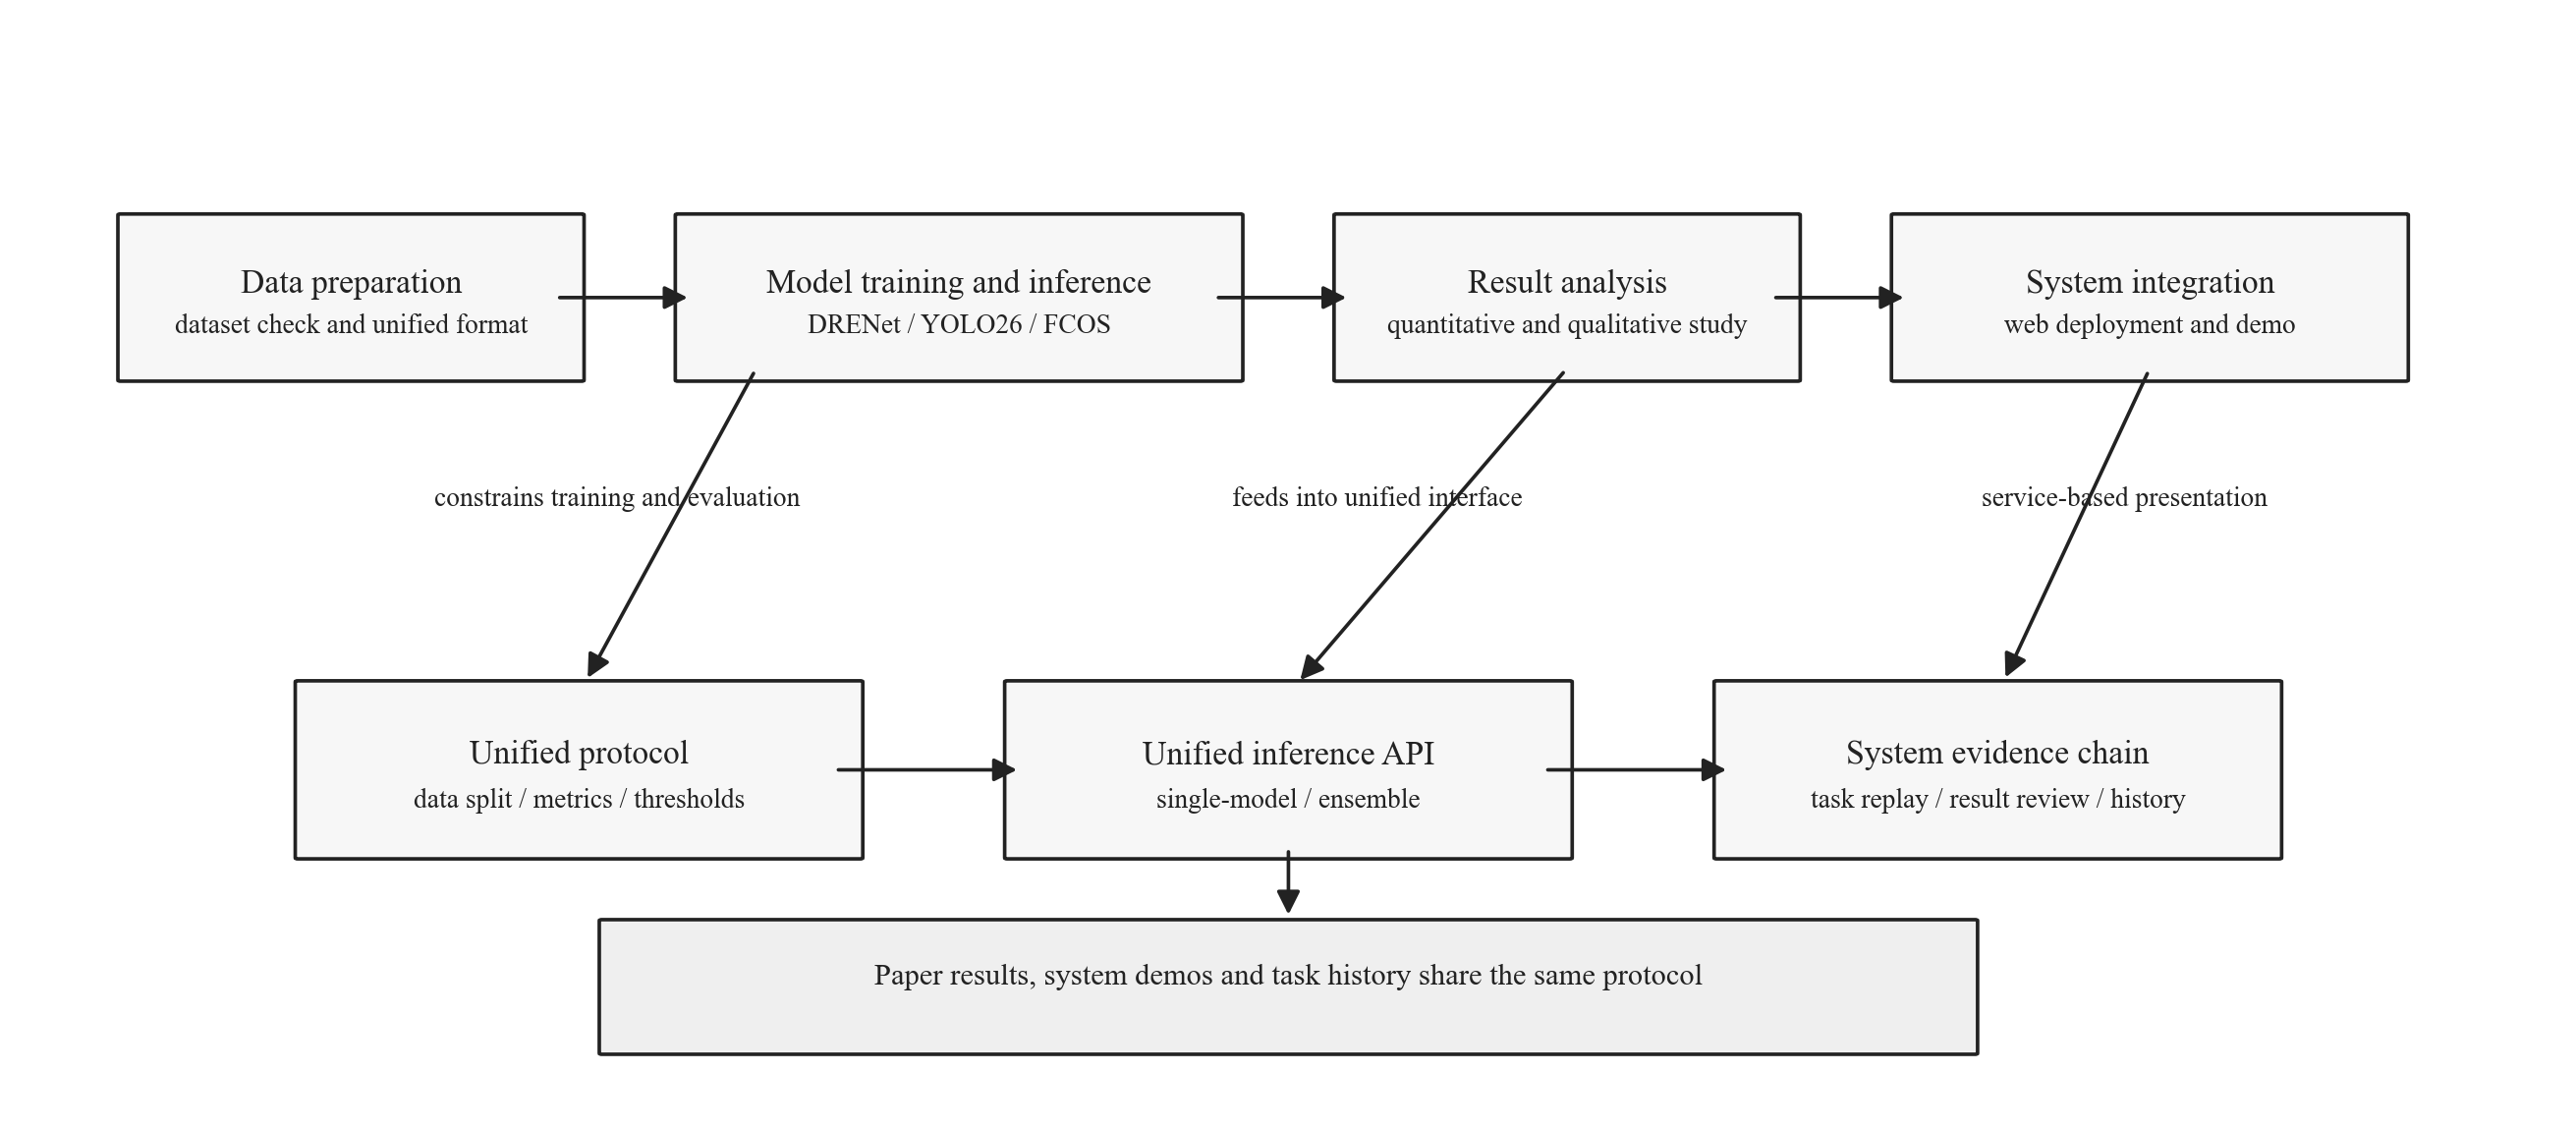
\includegraphics[width=0.96\textwidth]{img/ch1_pipeline.png}
  \caption{技术路线示意}
  \label{fig:ch1_pipeline}
\end{figure}

具体做法上，数据部分先检查图像与标注是否对应，再整理成后续框架都能使用的中间格式。模型部分分别保留专项方法、anchor-free 方法和 one-stage 方法三个参照。分析阶段不只看 AP50，还结合误检样例、漏检样例和消融结果判断模型行为。系统阶段则检查这些推理能力能否在真实任务提交、状态查询和结果展示流程中稳定运行。

沿着这条路线，本文最终保留了三类产物：LEVIR-Ship 上的数据与评测记录，DRENet/FCOS/YOLO26 的对比结果及误差分析，以及一个可本地运行的轻量级 Web 检测系统。后文各章围绕这三类产物展开。

\subsection{论文结构安排}

全文共分为六章，各章内容安排如下。

\begin{enumerate}
  \item 第一章为绪论，介绍研究背景、问题挑战、研究目标、主要工作以及技术路线；
  \item 第二章为国内外研究现状，梳理通用目标检测、小目标检测与遥感船舶检测相关研究，并明确本文切入点；
  \item 第三章介绍数据集、评价指标与方法方案，说明统一实验协议、模型选择依据以及实现约束；
  \item 第四章给出实验结果与分析，展示三模型主对比结果、效率对比、定性样例与消融实验；
  \item 第五章介绍系统需求分析、总体设计与实现过程，说明系统架构、数据库、接口与关键流程；
  \item 第六章为总结与展望，归纳全文工作，分析当前边界，并给出后续研究方向。
\end{enumerate}

\subsection{小结}

本章交代了课题背景、任务难点、工作目标和技术路线。遥感微小船舶检测在本文中既是模型比较问题，也是结果能否复查、系统能否跑通的问题。后续章节依次讨论相关研究、实验设置、结果分析和系统实现。
